%Traditional machine learning focuses on learning patterns from sets of (sometimes labelled) examples. 
%This is useful for learning approximations of concepts. % bad sentence
%However, for logical structures such as automata or propositional formulas, slight changes can result in very different behaviors. 
%It is not generally possible to exactly learn these structures from just labelled examples. 

Inductive synthesis or inductive learning 
is the synthesis of programs (concepts) from examples or other observations. 
Inductive synthesis has found application in formal methods, program analysis,
software engineering, and related areas, for problems such as 
invariant generation (e.g.~\cite{garg2014ice}),
program synthesis (e.g.,~\cite{solar2006combinatorial}),
and compositional reasoning (e.g.~\cite{cobleigh2003learning}).
Most inductive synthesis follows the query-based learning model, where the
%Therefore, researchers have introduced the active learning model, where the
learner is allowed to make queries about the target concept to an oracle. 
%%% commented out below since we also consider PAC learning
%Further, this typically falls in the setting of {\em exact learning}, where a concept (program)
%that is learned from oracle interactions must be correct -- i.e., an approximate or mostly-correct result is not enough.
Using the correct set of oracles can result in the polynomial time learnability of otherwise unlearnable sets \cite{angluin1988queries}. 
Using queries for software analysis is becoming increasingly popular (e.g., \cite{vaandrager17,howar2018active}).
The special nature of query-based learning for formal synthesis, where a program is automatically generated to fit a high-level specification through interaction with oracles,
has also been formalized \cite{jha2017theory}. 

%This has been particularly useful in paradigms such as 
%counter-example guided inductive synthesis \cite{solar2006combinatorial}.

In spite of this progress,
most algorithms for inductive learning/synthesis are monolithic; that is, even
if the concept (program) is made up of components, the algorithms seek to
learn the entire concept from interaction with an oracle.
In contrast, in this paper, we study the setting of {\em modular concept learning},
where a learning problem is analyzed by breaking it into independent components. 
If an element's membership in a concept depends solely on its membership in the 
components that make up the concept, 
learning the concept as a whole can be reduced to learning the components. 
We study concepts that are the Cartesian products (i.e., cross-products) of their 
component concepts. Such concept arise in several applications: 
(i) in invariant generation, an invariant that is the conjunction of other component
invariants;
(ii) in compositional reasoning, an automaton that is the product of individual automata encapsulating different aspects of an environment model, and
(iii) in program synthesis, a product program whose state space is the product of the state spaces of individual component programs.
%This can be thought of as learning conjunctions in that an element is part of a target concept if and only if its relevant variables are all of the component concepts. \todo{Is this clear? Should we be more explicit about the independent variable / concept class connection?}
Modular concept learning can improve the {\em efficiency} of learning since the complexity of several
query-based learning algorithms depends on the size of the concept (e.g. automaton) to
be learned, and, as is well known, this can grow exponentially with the number of components.
Besides improving efficiency of learning, from a software engineering perspective,
modular concept learning also has the
advantage of {\em reuse} of component learning algorithms.

We will focus on the oracle queries given in Table \ref{table:queries} and show several results, including both upper and lower bounds. 
We show learning cross-products from superset queries is no more difficult than learning each individual concept. 
Learning cross-products from equivalence queries or subset queries is intractable, while learning from just membership queries is polynomial, though somewhat expensive. 
We show that when a learning algorithm is allowed to make membership queries and is give a single positive example, previously intractable problems become tractable. 
We show that learning the disjoint unions of sets is easy.
Finally, we discuss the computational complexity of PAC-learning and show how it can be improved when membership queries are allowed. 

\begin{table}
\begin{center}
  \begin{tabularx}{\textwidth}{| c | c | c | X | }
    \hline
    Query Name & Symbol & Complexity & Oracle Definition \\ \hline
    Single Positive Query & $\oneposQ$ & $\oneposC(c)$ & Return a fixed $x \in c^*$ \\ \hline
    Positive Query & $\posQ$ & $\posC(c)$ & Return an $x\in c^*$ that has not yet been given as a positive example (if one exists)\\ \hline
    Membership Query & $\memQ$ & $\memC(c)$ & Given string $s$, return true iff $s \in c^*$ \\ \hline
    Equivalence Query & $\eqQ$ & $\eqC(c)$ & Given $c \in C$, return true if $c=c^*$ otherwise return $x \in (c \backslash c^*) \cup (c^* \backslash c)$\\ \hline 
    Subset Query & $\subQ$ & $\subC(c)$ & Given $c \in C$, return `true' if $c \subseteq c^*$ \mbox{  } otherwise return some $x \in c \backslash c^*$ \\ \hline
    Superset Query & $\supQ$ & $\supC(c)$ & Given $c \in C$, return `true' if $c \supseteq c^*$  otherwise return some $x \in c^* \backslash c$\\ \hline
    Example Query & $\pacQ_\dist$ & $\pacC(c, \dist)$ & Samples $x$ from $\dist$ and returns $x$ with a label indicating whether $x \in c^*$. \\ \hline
  \end{tabularx}
\end{center}
\caption{Types of queries studied in this paper.}
\label{table:queries}
\end{table}

\subsection{A Motivating Example}

%\begin{figure}
%\centering
%\begin{varwidth}{\linewidth}
%\begin{lstlisting}
    %int x = ??;
    %int y = ??;
    %int a = f(x);
    %int b = g(y);
    %
    %$\Phi = \phi_1(a) \wedge \phi_2(b)$
%\end{lstlisting}
%\end{varwidth}
%\caption{A simple partial program to be synthesized to satisfy a specification $\Phi$}
%\label{sketch}
%\end{figure}

\begin{figure}[h]
\centering
%\subfloat[(a)]{
\begin{minipage}[b]{0.4 \textwidth}
%\begin{varwidth}{\linewidth}
\begin{lstlisting}
    int x = ??;
    int y = ??;
    int a = f(x);
    int b = g(y);
    
    $\Phi = \phi_1(a) \wedge \phi_2(b)$
\end{lstlisting}
\end{minipage}
%\label{sketch}}
%\end{varwidth}
\qquad
%\subfloat[(b)]{
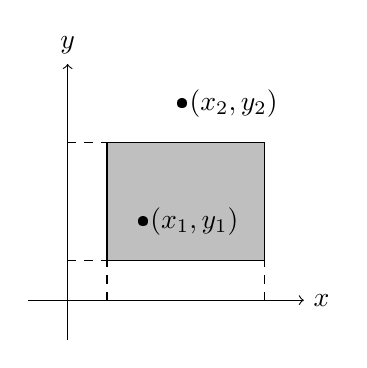
\begin{tikzpicture}
     \coordinate (BL) at (0.5,0.5);
     \coordinate (TR) at (2.5,2);
      \draw[->] (-0.5,0) -- (3,0) node[right] {$x$};
      \draw[->] (0,-0.5) -- (0,3) node[above] {$y$};
      \draw [draw=black] (BL) rectangle (TR);
      \filldraw [fill=lightgray, draw=black] (BL) rectangle (TR);
      \draw[dashed] (0,0.5) -- (BL);
      \draw[dashed] (0,2) -- (0.5,2);
      \draw[dashed] (0.5,0) -- (BL);
      \draw[dashed] (2.5,0) -- (2.5,0.5);
      \draw(.75,1) node[anchor = west]{\textbullet $(x_1,y_1)$};
      \draw(1.25,2.5) node[anchor = west]{\textbullet $(x_2,y_2)$};
      %\draw (1,1) node[draw=black, anchor=south] {.};
      %\tkzDefPoint(1,1){A};
      %\tkzLabelPoint[above](A){$(1,1)$};
\end{tikzpicture}
\caption{A simple partial program to be synthesized to satisfy a specification $\Phi$ (left) and the correct set of initial values for $x$ and $y$ (right).}
\label{sketch}
\label{sketchsolutions}
\end{figure}

To illustrate the learning problem, consider the sketching problem given in Figure \ref{sketch}.
Say we wanted to find the set of possible initial values for $x$ and $y$ that can replace the $??$ values so that the program satisfies $\Phi$.

Looking at the structure of this program and specification, we can see that the correctness of these two variables are independent of each other. 
Correct $x$ values are correct independent of $y$ and vice-versa.
Therefore, the set of settings will be the cross product of the acceptable settings for each variable.  
If an oracle can answer queries about correct $x$ or $y$ values separately, then the oracle can simply learn the acceptable values separately and take their Cartesian product. 

%\begin{figure}
%\begin{tikzpicture}
     %\coordinate (BL) at (0.5,0.5);
     %\coordinate (TR) at (2.5,2);
      %\draw[->] (-0.5,0) -- (3,0) node[right] {$x$};
      %\draw[->] (0,-0.5) -- (0,3) node[above] {$y$};
      %\draw [draw=black] (BL) rectangle (TR);
      %\filldraw [fill=lightgray, draw=black] (BL) rectangle (TR);
      %\draw[dashed] (0,0.5) -- (BL);
      %\draw[dashed] (0,2) -- (0.5,2);
      %\draw[dashed] (0.5,0) -- (BL);
      %\draw[dashed] (2.5,0) -- (2.5,0.5);
      %\draw(.75,1) node[anchor = west]{\textbullet $(x_1,y_1)$};
      %\draw(1.25,2.5) node[anchor = west]{\textbullet $(x_2,y_2)$};
      %%\draw (1,1) node[draw=black, anchor=south] {.};
      %%\tkzDefPoint(1,1){A};
      %%\tkzLabelPoint[above](A){$(1,1)$};
      %
%\end{tikzpicture}
%\caption{The correct set of initial values for $x$ and $y$.}
%\label{sketchsolutions}
%\end{figure}


If the correct values form intervals, the correct settings will look something like the rectangle shown in Figure \ref{sketchsolutions}.
An algorithm for learning this rectangle can try to simulate learning algorithms for each interval by acting as the oracle for each sublearner. 
For example, if both sublearners need a positive example, the learner can query the oracle for a positive example. 
Given the example $(x_1,y_1)$ as shown in the figure, the learner can then pass $x_1$ and $y_1$ to the sublearners as positive examples. 
However, this does not apply to negative examples, such as $(x_2, y_2)$ in the figure. 
In this example, $x_2$ is in its target interval, but $y_2$ is not. 
The learner has no way of knowing which subconcept a negative element fails on.
Handling negative counterexamples is one of the main challenges of this paper.




